\title{Dokumentacja projektu}
\author{
	Krzysztof Mizgała 262839
	\and 
	Maciej Kosierb 262239
	\and
	Wiktoria Kudła 262254
	\and
	Wiktoria Gałdusińska 262209
}
\date{\today}

\documentclass[12pt]{article}
\usepackage{hyperref}
\usepackage{polski}
\usepackage[utf8]{inputenc}
\usepackage{pgf-umlcd}
\usepackage{listings}

\begin{document}
	\maketitle
	
	\section{Opis projektu}\label{sec:opis-projektu}
	Nasza aplikacja służy do analizy danych finansowych.
	Korzysta z danych z https://site.financialmodelingprep.com/developer/docs/.
	Klucz API jest wymagany do uruchomienia aplikacji.
	Można go pobrać \href{https://site.financialmodelingprep.com/login}{tutaj} a następnie
	trzeba ustawić zmienną środowiskową API\_KEY do klucza.
	Można także korzystać z własnego klucza API tworząc plik .env w katalogu głównym projektu i
	dodając zmienną API\_KEY z kluczem jako wartość.

	Aplikacja pozwala na odczyt danych finansowych danej firmy.
	Używając różnych metod do zanalizowania, pokazuje wyniki i przewiduje ceny rynkowe.

	\section{Użyte technologie}\label{sec:uzyte-echnologie}
	 \href{https://site.financialmodelingprep.com/developer/docs/} - API, z którego korzystamy.

	 Wykorzystane biblioteki Pythona:
	\begin{itemize}
		\item pandas
		\item requests
		\item dotenv
		\item PyQt5
	\end{itemize}

	Lista plików:
	\begin{itemize}
		\item analysis.py
		\item api.py
		\item docs.tex
		\item README.md
		\item requirements.txt
		\item ui.py
	\end{itemize}

	\section{Opis metod}\label{sec:uzyte-metody}
	\begin{itemize}
	\item \textit{ui.py}
		\begin{itemize}
			\item \lstinline{_get_symbols} - pobiera symbole i nazwy analizowanych obiektów z pliku CSV.
			\item `\_init\_it` - tworzy graficzny interfejs użytkownika.
			\item `update\_symbols` - aktualizuje listę skrótów, kiedy kategoria jest zmieniona.
			\item `update\_signal` - aktualizuje etykietę sygnału i kolor pudełka (?:)), kiedy sygnał jest zmieniony.
			\item `update\_indicators` - aktualizuje listę wskaźników, kiedy pola wyboru są zmienione.
			\item `update\_bins` - aktualizuje liczbę słupków histogramu.
			\item `analyze` - analizuje dane dla wybranego obiektu.
			Pokazuje wyniki w postaci tabeli i wykresu świecowego.
			\item `\_analyze` - zaczyna analizę w osobnym wątku po to, by zapobiec zacinaniu się interfejsowi.
			\item `draw\_plot` - tworzy wykres świecowy.
			\item `plot\_candles` - tworzy świece wykresu na osiach na podstawie dostarczonych danych.
			\item `plot\_indicators` - tworzy wykres wskaźników, które zostały wybrane przez użytkownika, na wykresie
			świecowym.
			\item `plot\_sma` - tworzy wykres wskaźników SMA na wykresie świecowym.
			\item `plot\_ema` - tworzy wykres wskaźników EMA na wykresie świecowym.
			\item `plot\_bollinger` - tworzy wykres wstęg Bollingera na wykresie świecowym.
			\item `plot\_rsi` - tworzy wykres wskaźników RSI na wykresie świecowym.
			\item `plot\_macd` - tworzy wykres wskaźników na wykresie świecowym.
			\item `plot\_stochastic` - tworzy wykres oscylatora stochastycznego na wykresie świecowym.
			\item `plot\_williams` - tworzy wykres \%R Williamsa.
		\end{itemize}
		\item \textit{analysis.py}
		\begin{itemize}
			\item `get\_signal` - otrzymuje sygnał na opierający się na wskaźnikach analizy techniczej.
			Bazuje na następujących zasadach:
			\begin{itemize}
				\item Kupno, gdy MACD przekracza linię sygnału z góry.
				\item Sprzedaż, gdy MACD przekracza linię sygnału z dołu.
				\item Kupno, gdy RSI jest mniejszy niż 30.
				\item Sprzedaż, gdy RSI jest większy niż 70.
				\item Kupno, gdy \%K (oscylator wolny) przekroczy \%D (oscylator szybki).
				\item Sprzedaż, gdy \%D przekroczy \%K.
				\item Kupno, gdy SMA jest większe od EMA.
				\item Sprzedaż, gdy SMA jest mniejsze od EMA.
				\item Kupno, gdy SMA jest większe od ceny instrumentu.
				\item Sprzedaż, gdy SMA jest mniejsze od ceny instrumentu.
				\item Kupno, gdy EMA jest większe od ceny od ceny instrumentu.
				\item Sprzedaż, gdy EMA jest mniejsze od ceny instrumentu.
			\end{itemize}
			\item `sma` - Prosta Średnia Krocząca (ang. SMA - Simple Moving Average), jest
			najbardziej podstawową średnią kroczącą.
			Oblicza się ją sumując ceny zamykające z ostatnich\textit{n} dni i dzieląc tę sumę przez \textit{n}.
			\item `ema` - Wykładnicza Średnia Krocząca (ang. EMA - Exponential Moving Average) jest rodzajem
			średniej kroczącej, która kładzie większy nacisk na nowszych danych.
			EMA jest bardziej wrażliwy na ostatnie zmiany w cenie.
			\item `bollinger` - Wstęgi Bollingera to wstęgi zmienności między średnią krocząca.
			Zmienność jest liczona za pomocą odchylenia standardowego, które zmienia się, kiedy
			zmiennośc rośnie lub maleje.
			Wstęgi automatycznie poszerzają się, kiedy zmienność rośnie i zwężają, gdy maleje.
			\item `rsi` - Wskaźnik Siły Względnej (ang. RSI - Relative Strength Index) jest wskaźnikiem
			dynamiki, który mierzy znaczenie ostatnich zmian cen, aby ocenić warunki wykupienia lub wyprzedania
			akcji lub innego kapitału.
			\item `macd` - Konwergencja/Dywergencja Średnich Kroczących (ang. Moving Average Convergence Divergence)
			to wskaźnik dynamiki trendów pokazujący zaleźność pomiędzy dwiema średnimi kroczącymi cen.
			\item `stochastic` - Oscylator Stochastyczny (ang. Stochastic Oscillator) jest wskaźnikiem dynamiki,
			który porównuje konkretną cenę zamykającą do zakresu jej cen na przestrzeni czasu.
			\item `williams` - \%R Williamsa to wskaźnik dynamiki. Jest oscylatorem, który pokazuje zależność obecnej
			ceny zamknięcia w relacji do maksymalnej i minimalnej ceny z poprzednich dni.
		\end{itemize}
		\item \textit{api.py}
			\begin{itemize}
				\item `\_get\_data` - tworzy ramkę danych lub plik JSON z danych z API dla danego adresu URL.
				\item `list\_category` - tworzy listę symboli danej kategorii.
				\item `get\_historical` - pobiera ceny historyczne oraz wolumen dla danej akcji, kryptowaluty, forexa
				lub zasobu.
				\item `get\_historical\_capitalization` - pobiera kapitalizację historyczną dla konkretnego symbolu
				akcji.
			\end{itemize}
	\end{itemize}

	\section{Diagram UML}\label{sec:diagram-uml}
	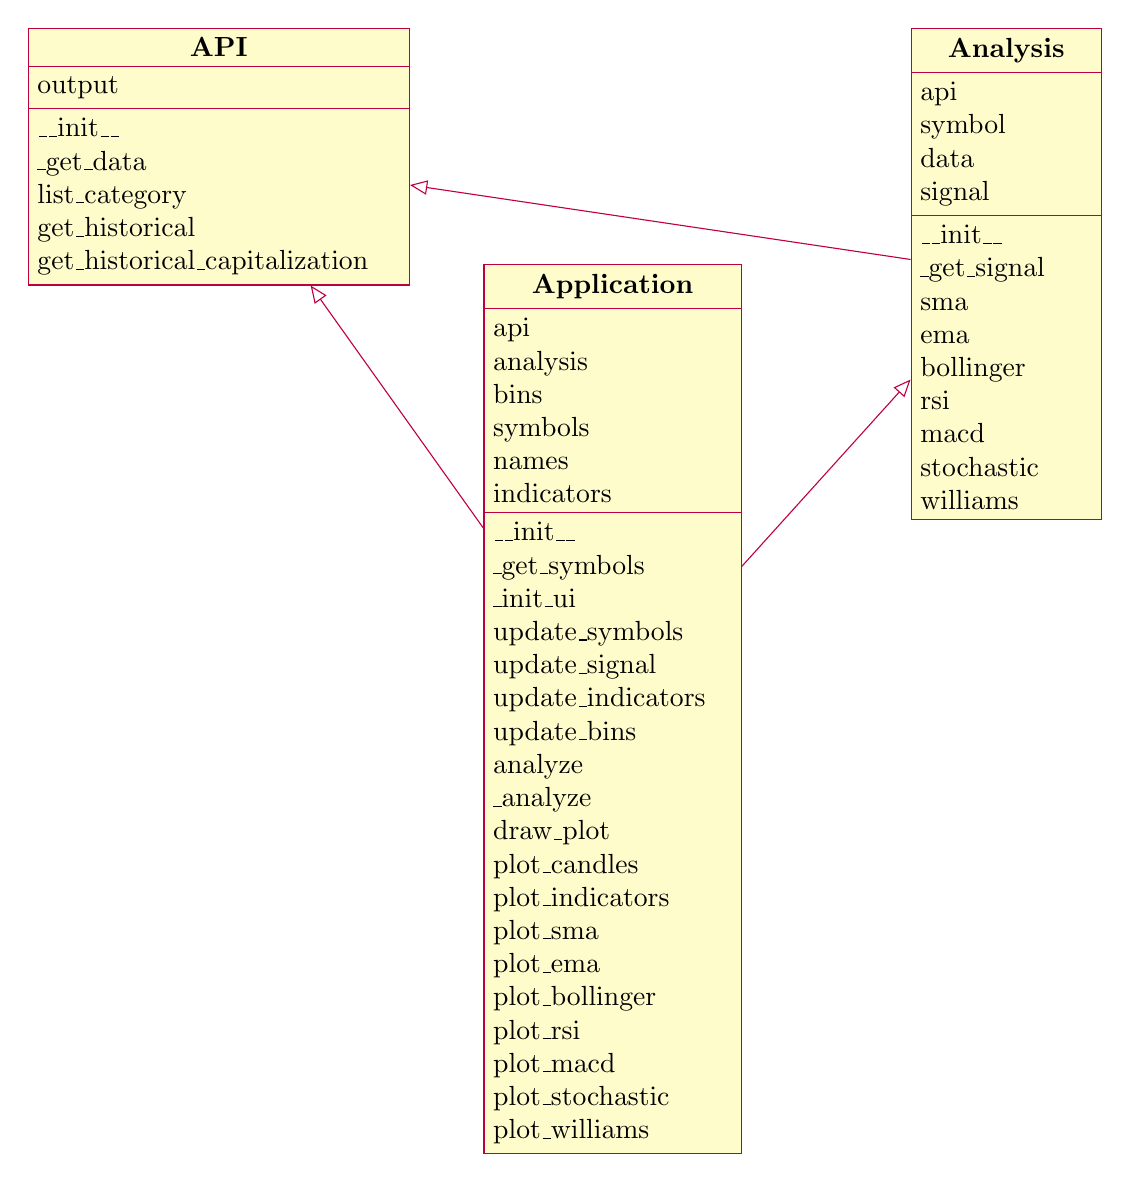
\begin{tikzpicture}
        \begin{class}[text width = 0.38\textwidth]{API}{0, 0}
            \attribute{output}
            \operation{\_\_init\_\_}
            \operation{\_get\_data}
            \operation{list\_category}
            \operation{get\_historical}
            \operation{get\_historical\_capitalization}
        \end{class}
        \begin{class}[text width = 0.18\textwidth]{Analysis}{10, 0}
            \inherit{API}
            \attribute{api}
            \attribute{symbol}
            \attribute{data}
            \attribute{signal}
            \operation{\_\_init\_\_}
            \operation{\_get\_signal}
            \operation{sma}
            \operation{ema}
            \operation{bollinger}
            \operation{rsi}
            \operation{macd}
            \operation{stochastic}
            \operation{williams}
        \end{class}
        \begin{class}[text width = 0.25\textwidth]{Application}{5, -3}
            \inherit{API}
            \inherit{Analysis}
            \attribute{api}
            \attribute{analysis}
            \attribute{bins}
            \attribute{symbols}
            \attribute{names}
            \attribute{indicators}
            \operation{\_\_init\_\_}
            \operation{\_get\_symbols}
            \operation{\_init\_ui}
            \operation{update\_symbols}
            \operation{update\_signal}
            \operation{update\_indicators}
            \operation{update\_bins}
            \operation{analyze}
            \operation{\_analyze}
            \operation{draw\_plot}
            \operation{plot\_candles}
            \operation{plot\_indicators}
            \operation{plot\_sma}
            \operation{plot\_ema}
            \operation{plot\_bollinger}
            \operation{plot\_rsi}
            \operation{plot\_macd}
            \operation{plot\_stochastic}
            \operation{plot\_williams}
        \end{class}
    \end{tikzpicture}

\end{document}
